\documentclass[14pt]{beamer} 
\usetheme{default}

\usepackage{import}
\usepackage{graphicx}

\usepackage{tikz}
\usetikzlibrary{shapes, arrows.meta}

\usepackage{pgfplots}
\usepackage[T1]{fontenc}
\usepackage{lmodern}
\usepackage[utf8]{inputenc}

%\setbeamercovered{transparent}
\definecolor{bgcol}{rgb}{0.8, 0.8, 0.8}
\setbeamercolor{bgcolor}{fg=black,bg=bgcol}

\newcommand{\concat}{\ensuremath{+\!\!\!\!+\,}}
\newcommand{\cov}{\vartriangleleft}
\newcommand{\unit}[1]{\ \text{#1}}
\newcommand{\nat}{\mathbb{N}}
\newcommand{\suchthat}{\ |\ }
\newcommand{\List}[1]{\mathsf{list}\ {#1}}
\newcommand{\rat}{\mathbb{Q}}
\newcommand{\R}{\mathbb{R}}
\newcommand{\bool}{\mathbb{B}}
\newcommand{\Prop}{\mathbb{P}}
\newcommand{\Dist}[1]{\mathcal{P}({#1})}
\newcommand{\fun}[2]{\lambda\ {#1}\Rightarrow{#2}}

\newcommand*\circled[1]{\tikz[baseline=(char.base)]{
            \node[shape=circle,draw,inner sep=2pt,thick] (char) {#1};}}

\title{Running and reasoning about continuous and probabilistic programs}
\author{Ben Sherman}
\date{May 31, 2016}

\setbeamertemplate{footline}{}
\setbeamertemplate{navigation symbols}{}
\setbeamertemplate{headline}
{\vspace{0.03em}
\begin{beamercolorbox}[wd=\paperwidth,ht=4ex,dp=1ex,center]{bgcolor}
 \small \insertshorttitle
  \end{beamercolorbox}
}
\begin{document}

\begin{frame}

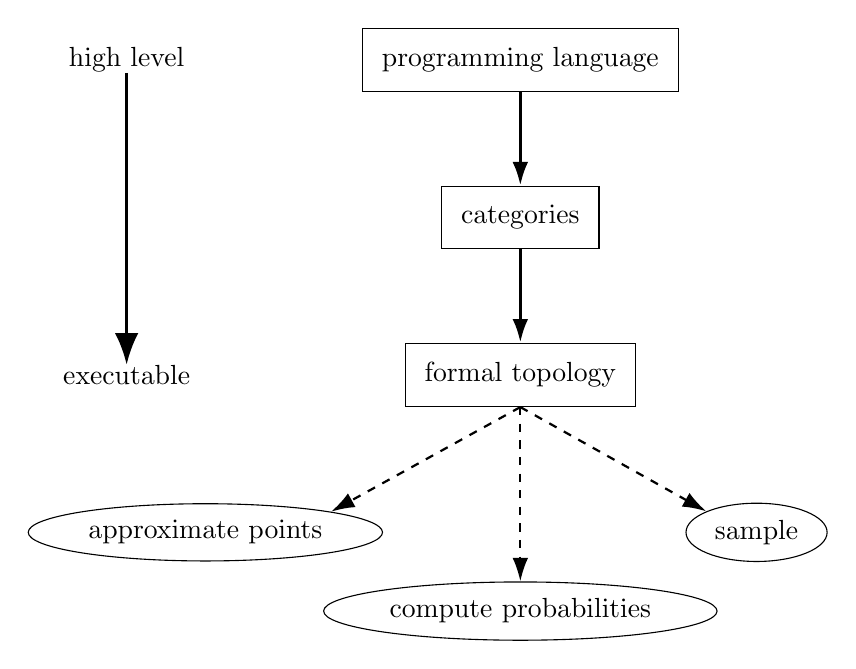
\begin{tikzpicture}
\node[inner sep=0pt] (highlevel) at (0,0)
  {high level};
\node[inner sep=0pt] (executable) at (0, -4)
  {executable};
\draw[-{Latex[length=4mm, width=3mm]},very thick] (highlevel.south) -- (executable.north);

\node[draw=black, rectangle, inner sep=7pt] (pl) at (5,0)
  {programming language};
\node[draw=black, rectangle, inner sep=7pt] (cat) at (5,-2)
  {categories};
\node[draw=black, rectangle, inner sep=7pt] (ft) at (5,-4)
  {formal topology};
  
\draw[-{Latex[length=3mm, width=2mm]},very thick] (pl.south) -- (cat.north);
\draw[-{Latex[length=3mm, width=2mm]},very thick] (cat.south) -- (ft.north);

\node[ellipse, draw=black, inner sep=3pt] (ex1) at (1,-6)
  {approximate points};
\node[ellipse, draw=black, inner sep=3pt] (ex2) at (5,-7)
  {compute probabilities};
\node[ellipse, draw=black, inner sep=3pt] (ex3) at (8,-6)
  {sample};
  
\draw[-{Latex[length=3mm, width=2mm]},thick, dashed] (ft.south) -- (ex1.north east);
\draw[-{Latex[length=3mm, width=2mm]},thick, dashed] (ft.south) -- (ex2.north);
\draw[-{Latex[length=3mm, width=2mm]},thick, dashed] (ft.south) -- (ex3.north west);

\end{tikzpicture}


\end{frame}


\begin{frame}
\[
\frac{x : \Gamma \leadsto \Dist{A} \qquad f : \Gamma \times A \leadsto \Dist{A}}
{\mathsf{stream}\ x\  f : \Gamma \leadsto \Dist{\mathsf{Stream}\ A}}
\]

\begin{align*}
ou &: \R \times \R \leadsto \Dist{\mathsf{Stream}\ \R}
\\
ou (\theta, \sigma) &= \mathsf{stream}\ (\mathsf{ret}\ 0) 
\\
 &(\fun{x}{ z \leftarrow \mathcal{N}(0, \sigma^2); \mathsf{ret}\  ((1 - \theta)x + z)})
\end{align*}

\begin{tikzpicture}
\node[inner sep=5pt] (step1) at (0,0)
    {\def\svgwidth{0.25\textwidth}
\import{../Figures/Cover/output/}{step1.pdf_tex}};
\node[inner sep=5pt] (step2) at (4,0)
    {\def\svgwidth{0.25\textwidth}
    \import{../Figures/Cover/output/}{step2.pdf_tex}};
\node[inner sep=5pt] (step3) at (8,0)
    {\def\svgwidth{0.25\textwidth}
    \import{../Figures/Cover/output/}{step3.pdf_tex}};
\draw[double, -{Latex[length=4mm, width=3mm]},very thick] (step1.east) -- (step2.west);
\draw[double, -{Latex[length=4mm, width=3mm]},very thick] (step2.east) -- (step3.west);
\end{tikzpicture}
\end{frame}

\end{document}

